\documentclass{article}
\usepackage[UTF8]{ctex}
\usepackage{enumitem}
\usepackage{graphicx}
\usepackage{float}
\usepackage{subfigure}
\usepackage{amsmath,amsfonts}
\usepackage{hyperref}
\usepackage{listings}

\begin{document}
\sloppy % 解决中英文混排的断行问题

\title{编译实验心得报告}
\author{郑泓东 21311570}
\date{\today}

\maketitle

\section{编译器代码阅读技巧}
由于课程中的代码并不是由我们自己一步一步写出来的,而是由老师提供的,因此,代码中的各种结构体、函数等等,不是一时半会就能理解的。同时,由于课程实验的战线拉得比较长,而每个星期只有一节实验课,如果我们没有将课余时间分配给实验课得话,那么,上一星期才勉强看懂的代码,往往在下一星期就忘得一干二净了。

所以,我们需要一边看代码,一边做笔记。对于各种结构体,最好能画出它们的结构图,这样,我们在阅读代码的时候,就能更加清晰地知道它们之间的关系。对于各种函数,最好能写出它们的功能,这样,我们在阅读代码的时候,就能更加清晰地知道它们的作用。

\section{编译器代码编写调试心得}

\subsection{Makefile}
在实验过程中,我们需要不断地修改代码,然后编译运行,如果每次都手动输入编译命令,那么,效率会非常低。因此,我们需要学会使用 Makefile 来自动化编译运行的过程。而老师提供的 Makefile 文件往往只包含基本的编译命令。

我们往往需要添加一些自己的编译命令,比如,添加对某个文件的测试等等。因此,我建议在实验开始之前,学习一下 Makefile 的简单用法。

\subsection{Git}
通过观察 Git 仓库的提交记录,我们可以清晰地看到每次提交的内容,这样,我们就可以更加方便地进行代码的回退。同时,我们也可以对比不同版本之间的代码。以 Lab 4 - 目标代码生成为例:编译输出的汇编代码往往是一大堆,如果我们想要找到修改的代码对输出的汇编代码的影响,无疑是大海捞针。而通过 Git,我们可以很方便地找到修改的代码(图\ref{fig:Git}),从而更加方便地进行调试。而多次使用 Git 提交代码,也能培养我们的代码规范意识。

\begin{figure}[h]
    \centering
    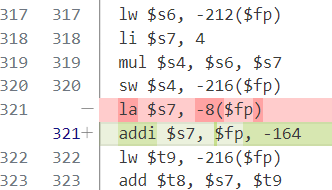
\includegraphics[width=0.5\textwidth]{../lab04-object-code-generation/pic/image-20231216110014714.png}
    \caption{Git}
    \label{fig:Git}
\end{figure}

\section{工具分享}

\subsection{适用于 Linux 的 Windows 子系统}

WSL2\footnote{WSL2: Windows Subsystem for Linux 2.}是 Windows 的一项功能,可用于在 Windows 计算机上运行 Linux 环境,而无需单独的虚拟机或双引导,旨在为希望同时使用 Windows 和 Linux 的开发人员提供无缝高效的体验。WSL2 相比于传统虚拟机的优势包括:
\begin{enumerate}
    \item 性能: WSL2 使用真实的 Linux 内核,而不是仿真,因此在性能方面表现更好。它通过轻量级的虚拟化技术( Hyper-V 虚拟机)实现,因此在访问文件系统和运行 Linux 应用程序时具有更低的延迟。
    \item 集成度: WSL2允许在Windows上运行本机的 Linux 二进制文件,而无需进行任何修改。这意味着你可以直接在 Windows 终端或其他终端模拟器中运行 Linux 命令,而无需启动完整的虚拟机。
    \item 与 Windows 集成: WSL2 可以更好地集成到 Windows 生态系统中。例如,你可以通过 Windows 资源管理器访问 WSL2 文件系统,并且可以在 Windows 和 Linux 之间轻松复制粘贴文本。
\end{enumerate}

\subsection{Ubuntu 包管理工具}
aptitude 是 Ubuntu 的包管理工具,可以用来安装、卸载、更新软件包。aptitude 在处理软件包依赖关系时比 apt-get 更加智能。它能够提供更好的解决方案,以确保软件的安装和卸载不会破坏系统的稳定性。

\section{其他心得}

\subsection{实验环境}
我在实验的过程中,使用的是 Windows 11 操作系统,通过 WSL2 安装了 Ubuntu 22.04.2 LTS,系统与各个软件的版本基本上在当时是最新的,也没有出现什么问题。实验环境的具体信息如下:

\begin{itemize}
    \item GNU Linux Release: Ubuntu 22.04.2 LTS, kernel version 5.15.133.1-microsoft-standard-WSL2
    \item GCC version 11.2.0
    \item GNU Flex version 2.6.4
    \item GNU Bison version 3.8.2
\end{itemize}

\subsection{降低内核版本}
如果确实想要保持和老师的实验环境一致,唯一的难点就是降低内核版本。这里提供一个降低内核版本的方法。

\href{https://blog.csdn.net/qq_49814035/article/details/116035670}{Ubuntu20.04 如何降低内核版本}

\section{课程建议}
我记得 Lab - 1 词法分析与语法分析的实验 PPT 上的编译命令是不编译 Tree.c (图\ref{fig:lab1})的。而实际操作中,编译命令应该带上 Tree.c。我猜是因为课程代码是基于完整的代码,挖出其中一部分,但又不好去掉 Tree.c 导致的。所以,建议在实验 PPT 上的编译命令中,都带上 Tree.c 的编译命令。或者可以补充说明一下,在此情此景下,为什么有 Tree.c 的文件,为什么必须要编译 Tree.c 。

\begin{figure}[h]
    \centering
    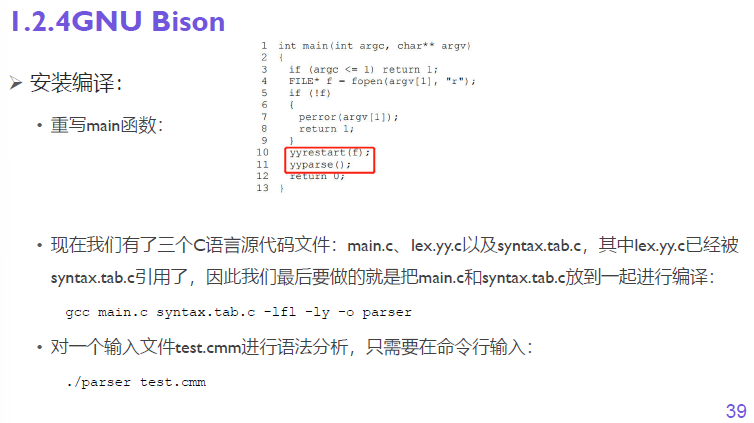
\includegraphics[width=1\textwidth]{pic/lab1.png}
    \caption{Lab - 1 词法分析与语法分析的实验 PPT 上的编译命令}
    \label{fig:lab1}
\end{figure}

理论课和实验课的割裂感还是比较强的,希望在实验课上,能够帮学生复习一下理论课上的知识,比如,词法分析、语法分析、语义分析、目标代码生成等等的原理。同时,理论课上,也可以提一嘴实验课上的知识,比如,在实验课上遇到的问题,以及在实验课上学到的知识。

\begin{figure}[h]
    \centering
    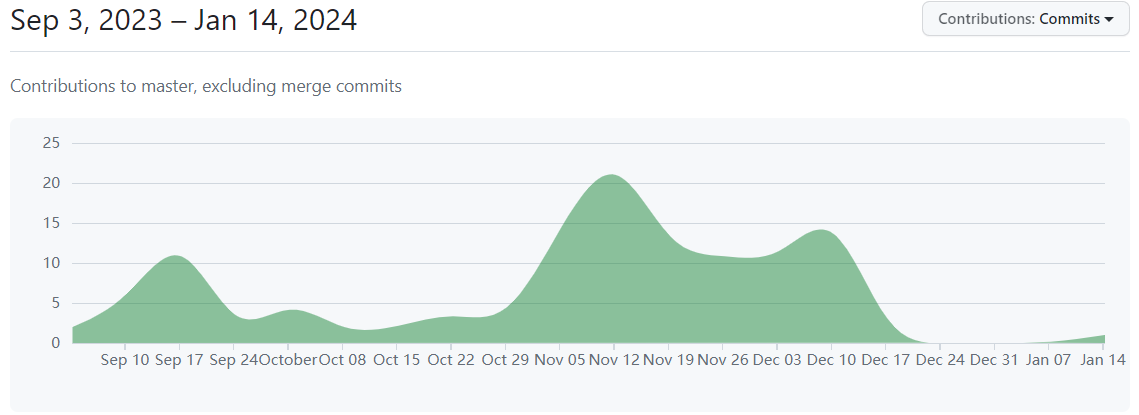
\includegraphics[width=1\textwidth]{pic/timeline.png}
    \caption{GitHub's timeline of commits}
    \label{fig:timeline}
\end{figure}

总的来说,编译器构造实验这门课还是比较痛苦的,但是编译成功、测试通过的那一刻,还是很有成就感的。从 GitHub 上的 commits 时间线(图\ref{fig:timeline})上,也能看出来,Lab 1 - 词法分析与语法分析、Lab 3 - 中间代码生成、Lab 4 - 目标代码生成的工作量是比较大的,而 Lab 2 - 语义分析则相对较小。所以,建议老师可以适当调整一下课程安排。



\end{document}
